\chapter{Protótipos de Baixa Fidelidade e Questionários}

\begin{itemize}

\item \textbf{Aplicação}

Assim, definidas as heurística e metodologia de produção do protótipo, fez-se o protótipo de baixa fidelidade
Protótipo de papel

\begin{figure}[h]
  \centering
  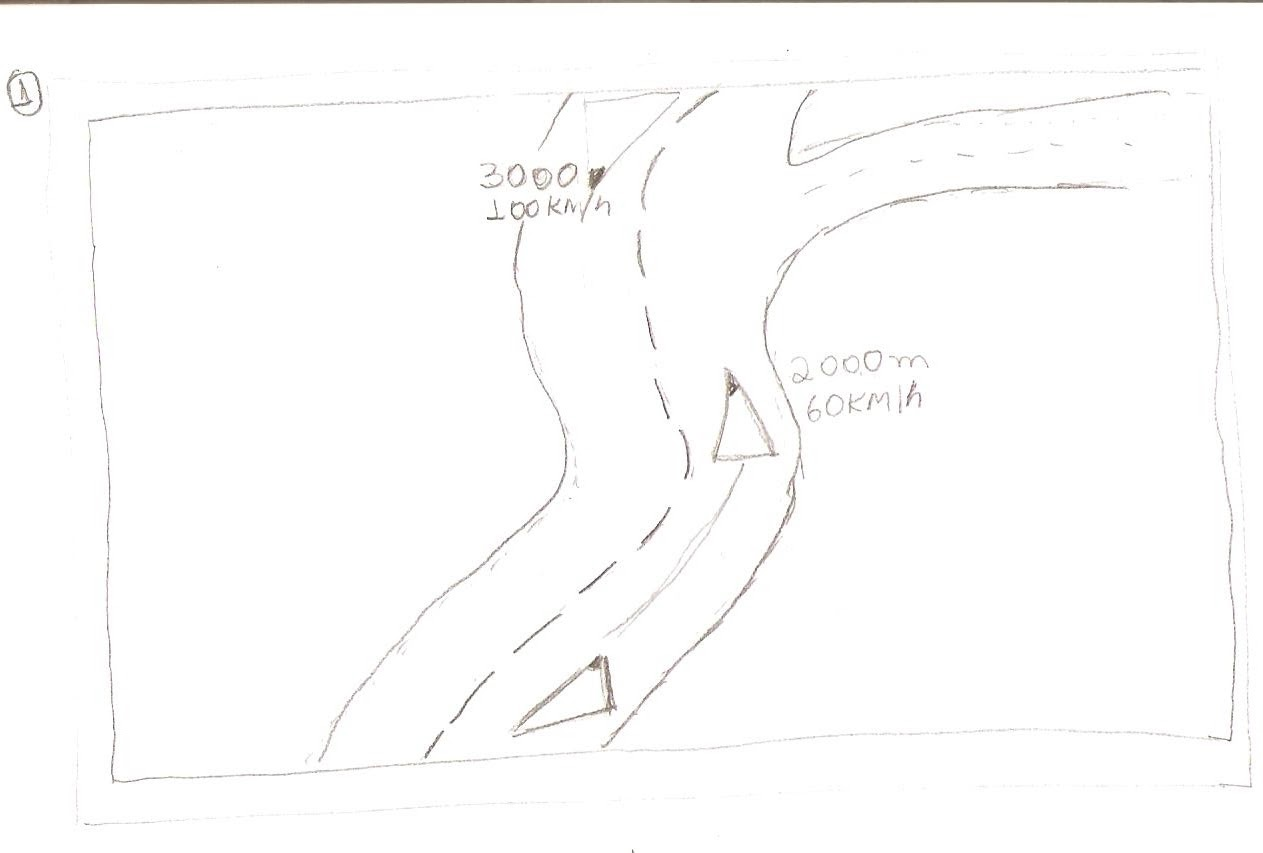
\includegraphics[width=300px, scale=1]{figuras/prototipo1}
  \caption{Protótipo de Papel 1}
\label{fig:prototipo1}
\end{figure}

\begin{figure}[h]
  \centering
  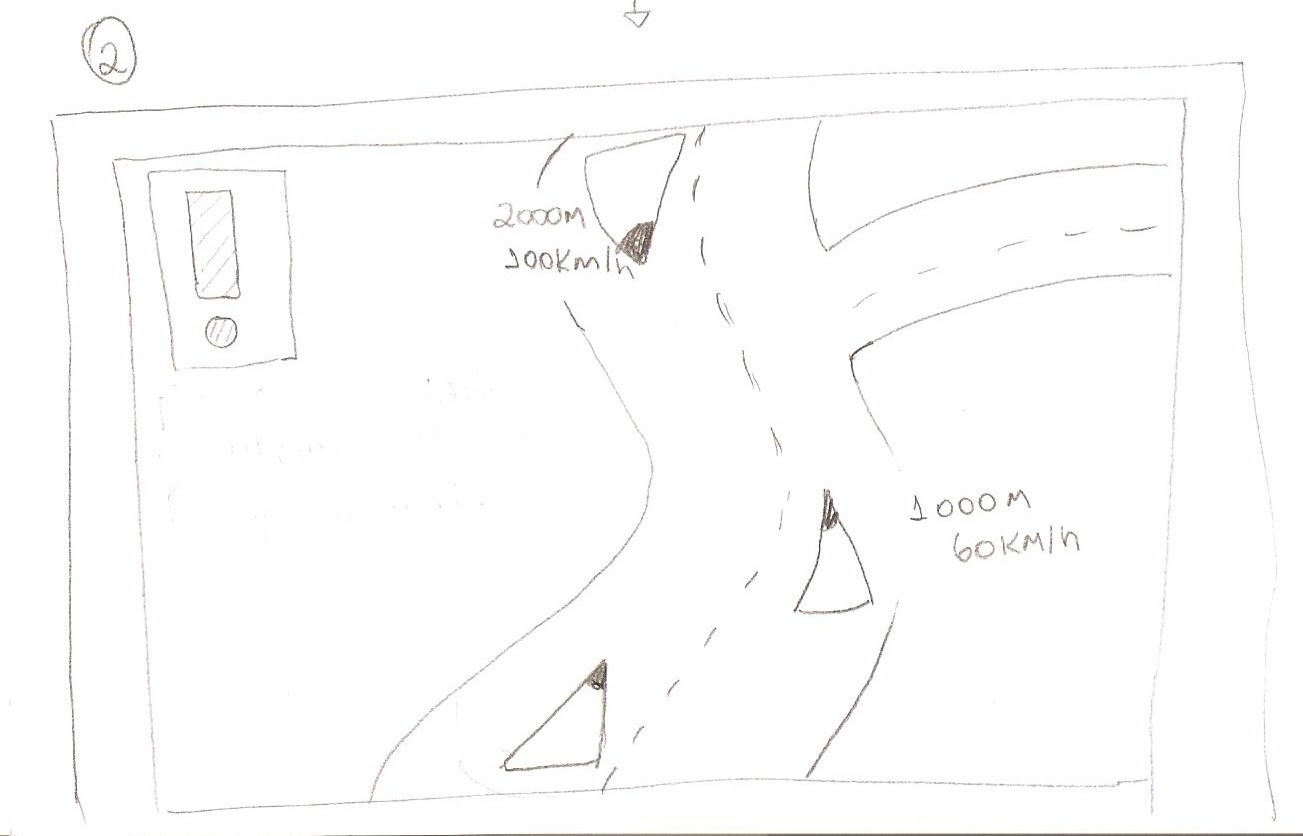
\includegraphics[width=300px, scale=1]{figuras/prototipo2}
  \caption{Protótipo de Papel 2}
\label{fig:prototipo2}
\end{figure}

\begin{figure}[h]
  \centering
  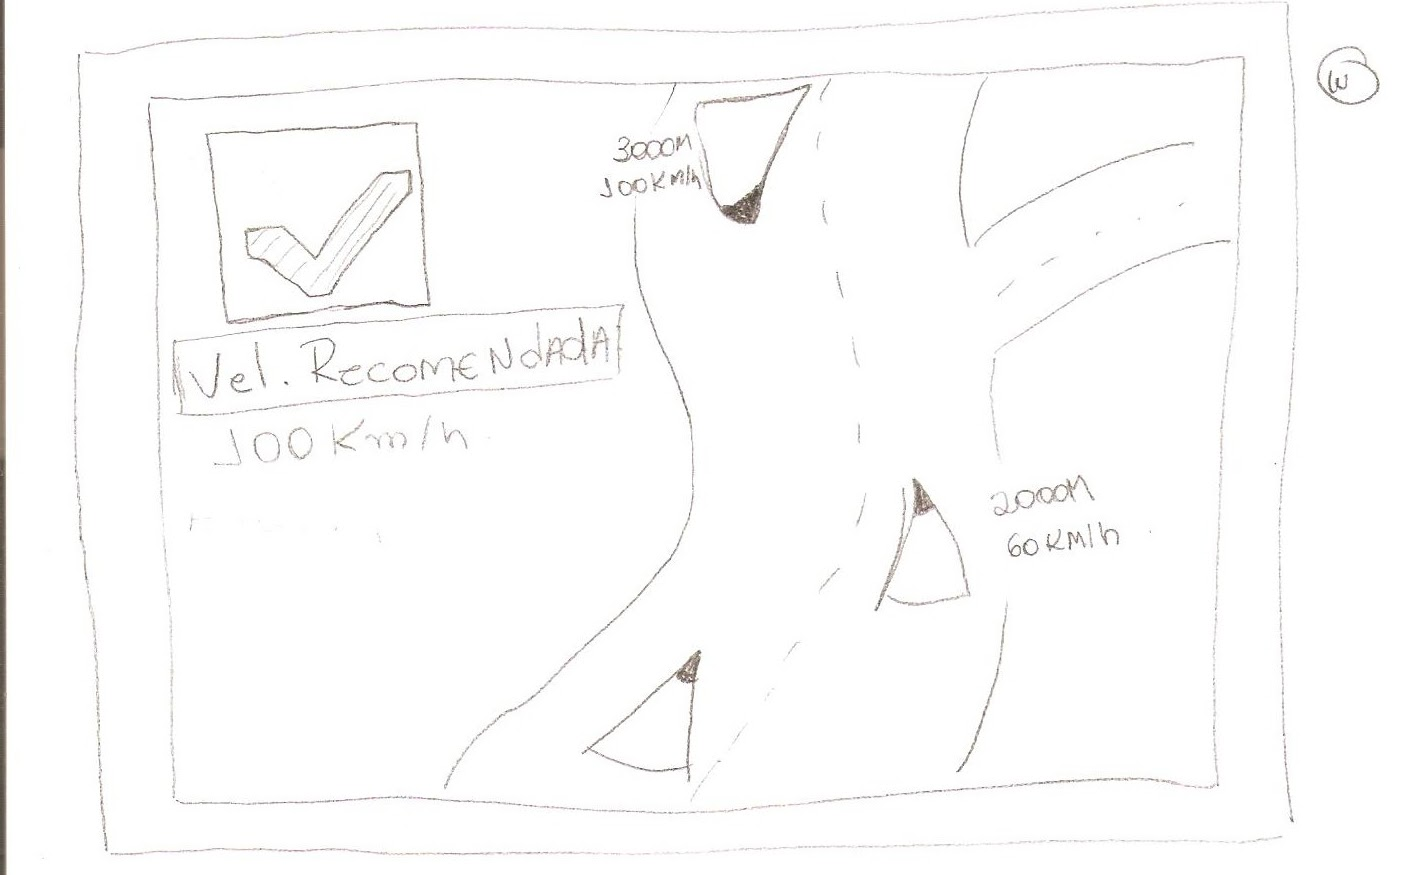
\includegraphics[width=300px, scale=1]{figuras/prototipo3}
  \caption{Protótipo de Papel 3}
\label{fig:prototipo3}
\end{figure}

Para maior proveito da avaliação, é desejável uma análise dos usuários avaliadores para adaptar a interface às suas vontades e desejos e construir um produto com alta possibilidades de sucesso. Para isto foram realizadas um grupo de perguntas para motoristas que apresentaram interesse no projeto. Abaixo seguem os resultados dos motoristas interessados no produto:

\begin{figure}[h]
  \centering
  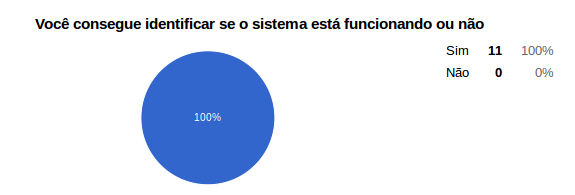
\includegraphics[width=300px, scale=1]{figuras/result1}
  \caption{Resultados da pergunta 1}
\label{fig:result1}
\end{figure}


\begin{figure}[h]
  \centering
  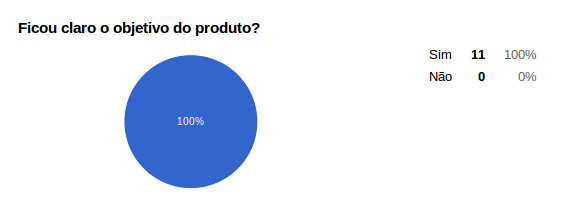
\includegraphics[width=300px, scale=1]{figuras/result2}
  \caption{Resultados da pergunta 2}
\label{fig:result2}
\end{figure}


\begin{figure}[h]
  \centering
  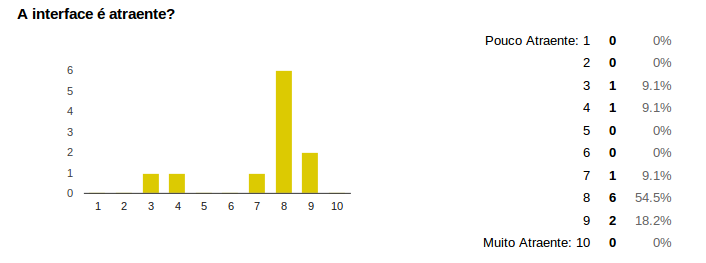
\includegraphics[width=300px, scale=1]{figuras/result3}
  \caption{Resultados da pergunta 3}
\label{fig:result3}
\end{figure}


\begin{figure}[h]
  \centering
  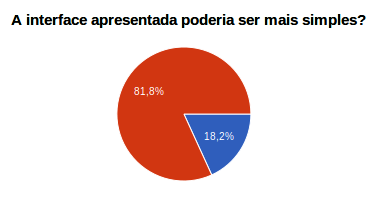
\includegraphics[width=300px, scale=1]{figuras/result4}
  \caption{Resultados da pergunta 4}
\label{fig:result4}
\end{figure}


\begin{figure}[h]
  \centering
  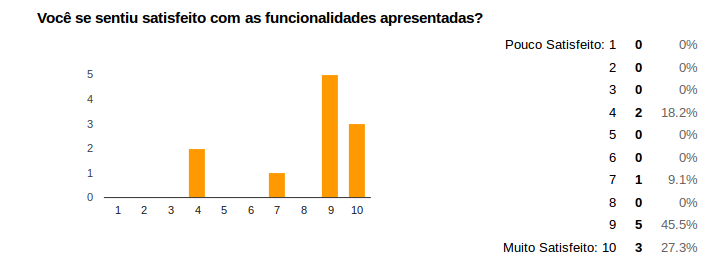
\includegraphics[width=300px, scale=1]{figuras/result5}
  \caption{Resultados da pergunta 5}
\label{fig:result5}
\end{figure}


\begin{figure}[h]
  \centering
  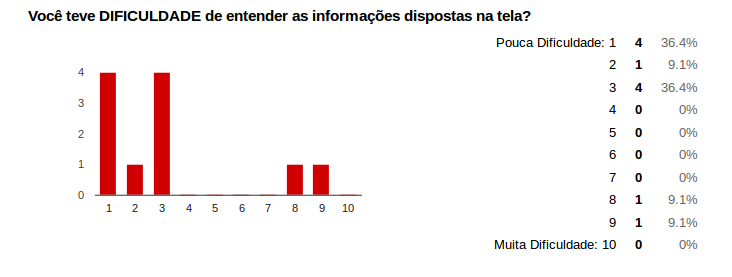
\includegraphics[width=300px, scale=1]{figuras/result6}
  \caption{Resultados da pergunta 6}
\label{fig:result6}
\end{figure}


\begin{figure}[h]
  \centering
  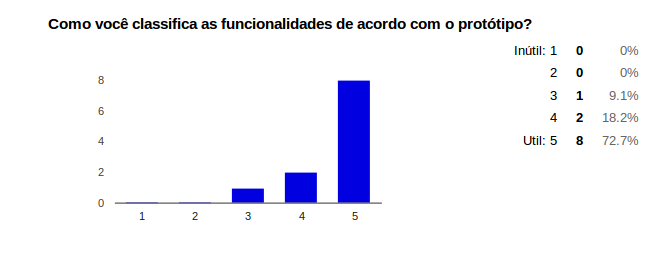
\includegraphics[width=300px, scale=1]{figuras/result7}
  \caption{Resultados da pergunta 7}
\label{fig:result7}
\end{figure}


\begin{figure}[h]
  \centering
  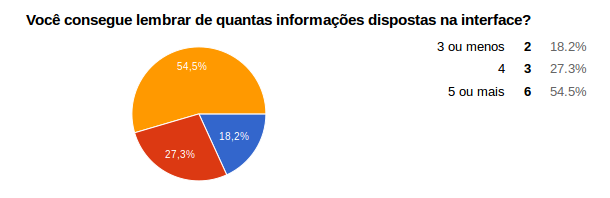
\includegraphics[width=300px, scale=1]{figuras/result8}
  \caption{Resultados da pergunta 8}
\label{fig:result8}
\end{figure}


\begin{figure}[h]
  \centering
  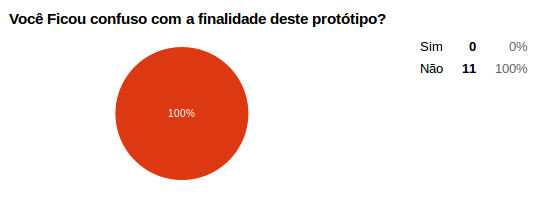
\includegraphics[width=300px, scale=1]{figuras/result9}
  \caption{Resultados da pergunta 9}
\label{fig:result9}
\end{figure}


\begin{figure}[h]
  \centering
  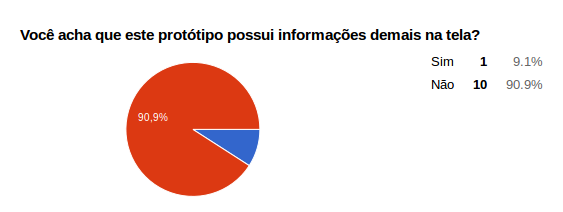
\includegraphics[width=300px, scale=1]{figuras/result10}
  \caption{Resultados da pergunta 10}
\label{fig:result10}
\end{figure}


\begin{figure}[h]
  \centering
  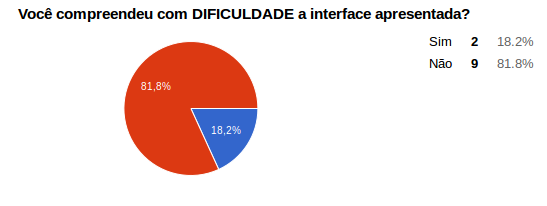
\includegraphics[width=300px, scale=1]{figuras/result11}
  \caption{Resultados da pergunta 11}
\label{fig:result11}
\end{figure}


\begin{figure}[h]
  \centering
  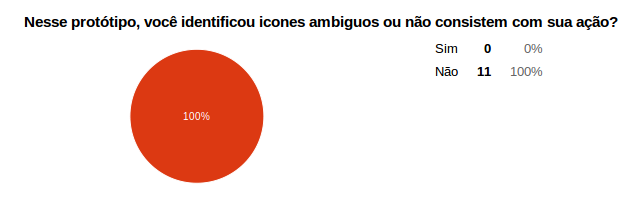
\includegraphics[width=300px, scale=1]{figuras/result12}
  \caption{Resultados da pergunta 12}
\label{fig:result12}
\end{figure}
	 	 	 	
\begin{figure}[h]
  \centering
  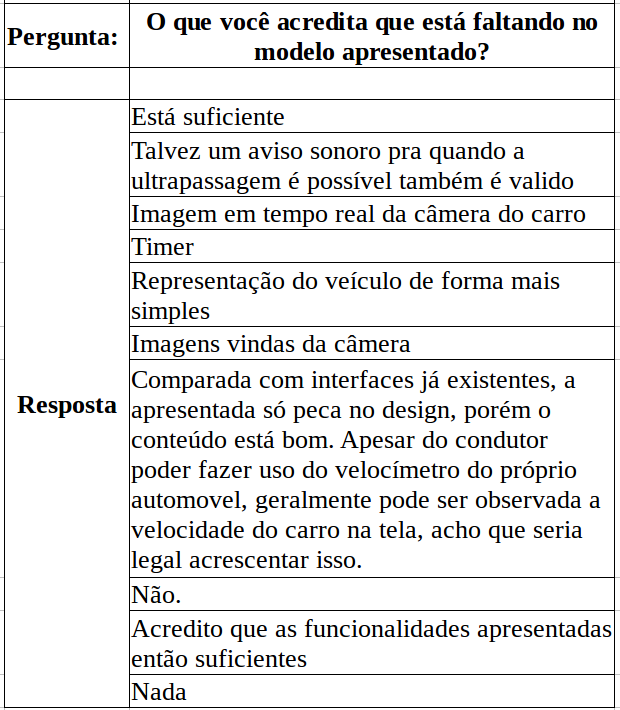
\includegraphics[width=300px, scale=1]{figuras/quadro1}
  \caption{Resultados da pergunta 13}
\label{fig:quadro1}
\end{figure}			

\begin{figure}[h]
  \centering
  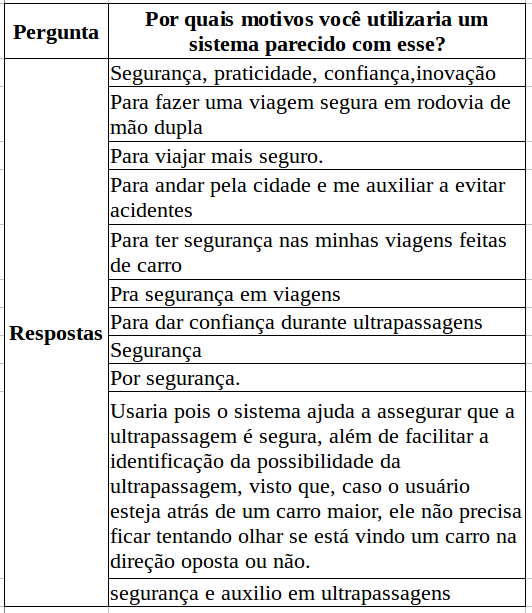
\includegraphics[width=300px, scale=1]{figuras/quadro2}
  \caption{Resultados da pergunta 14}
\label{fig:quadro2}
\end{figure}	

\end{itemize}